\begin{figure}[hp]
% 
\subcaptionbox{\label{fig:cluster22-Aa}}
{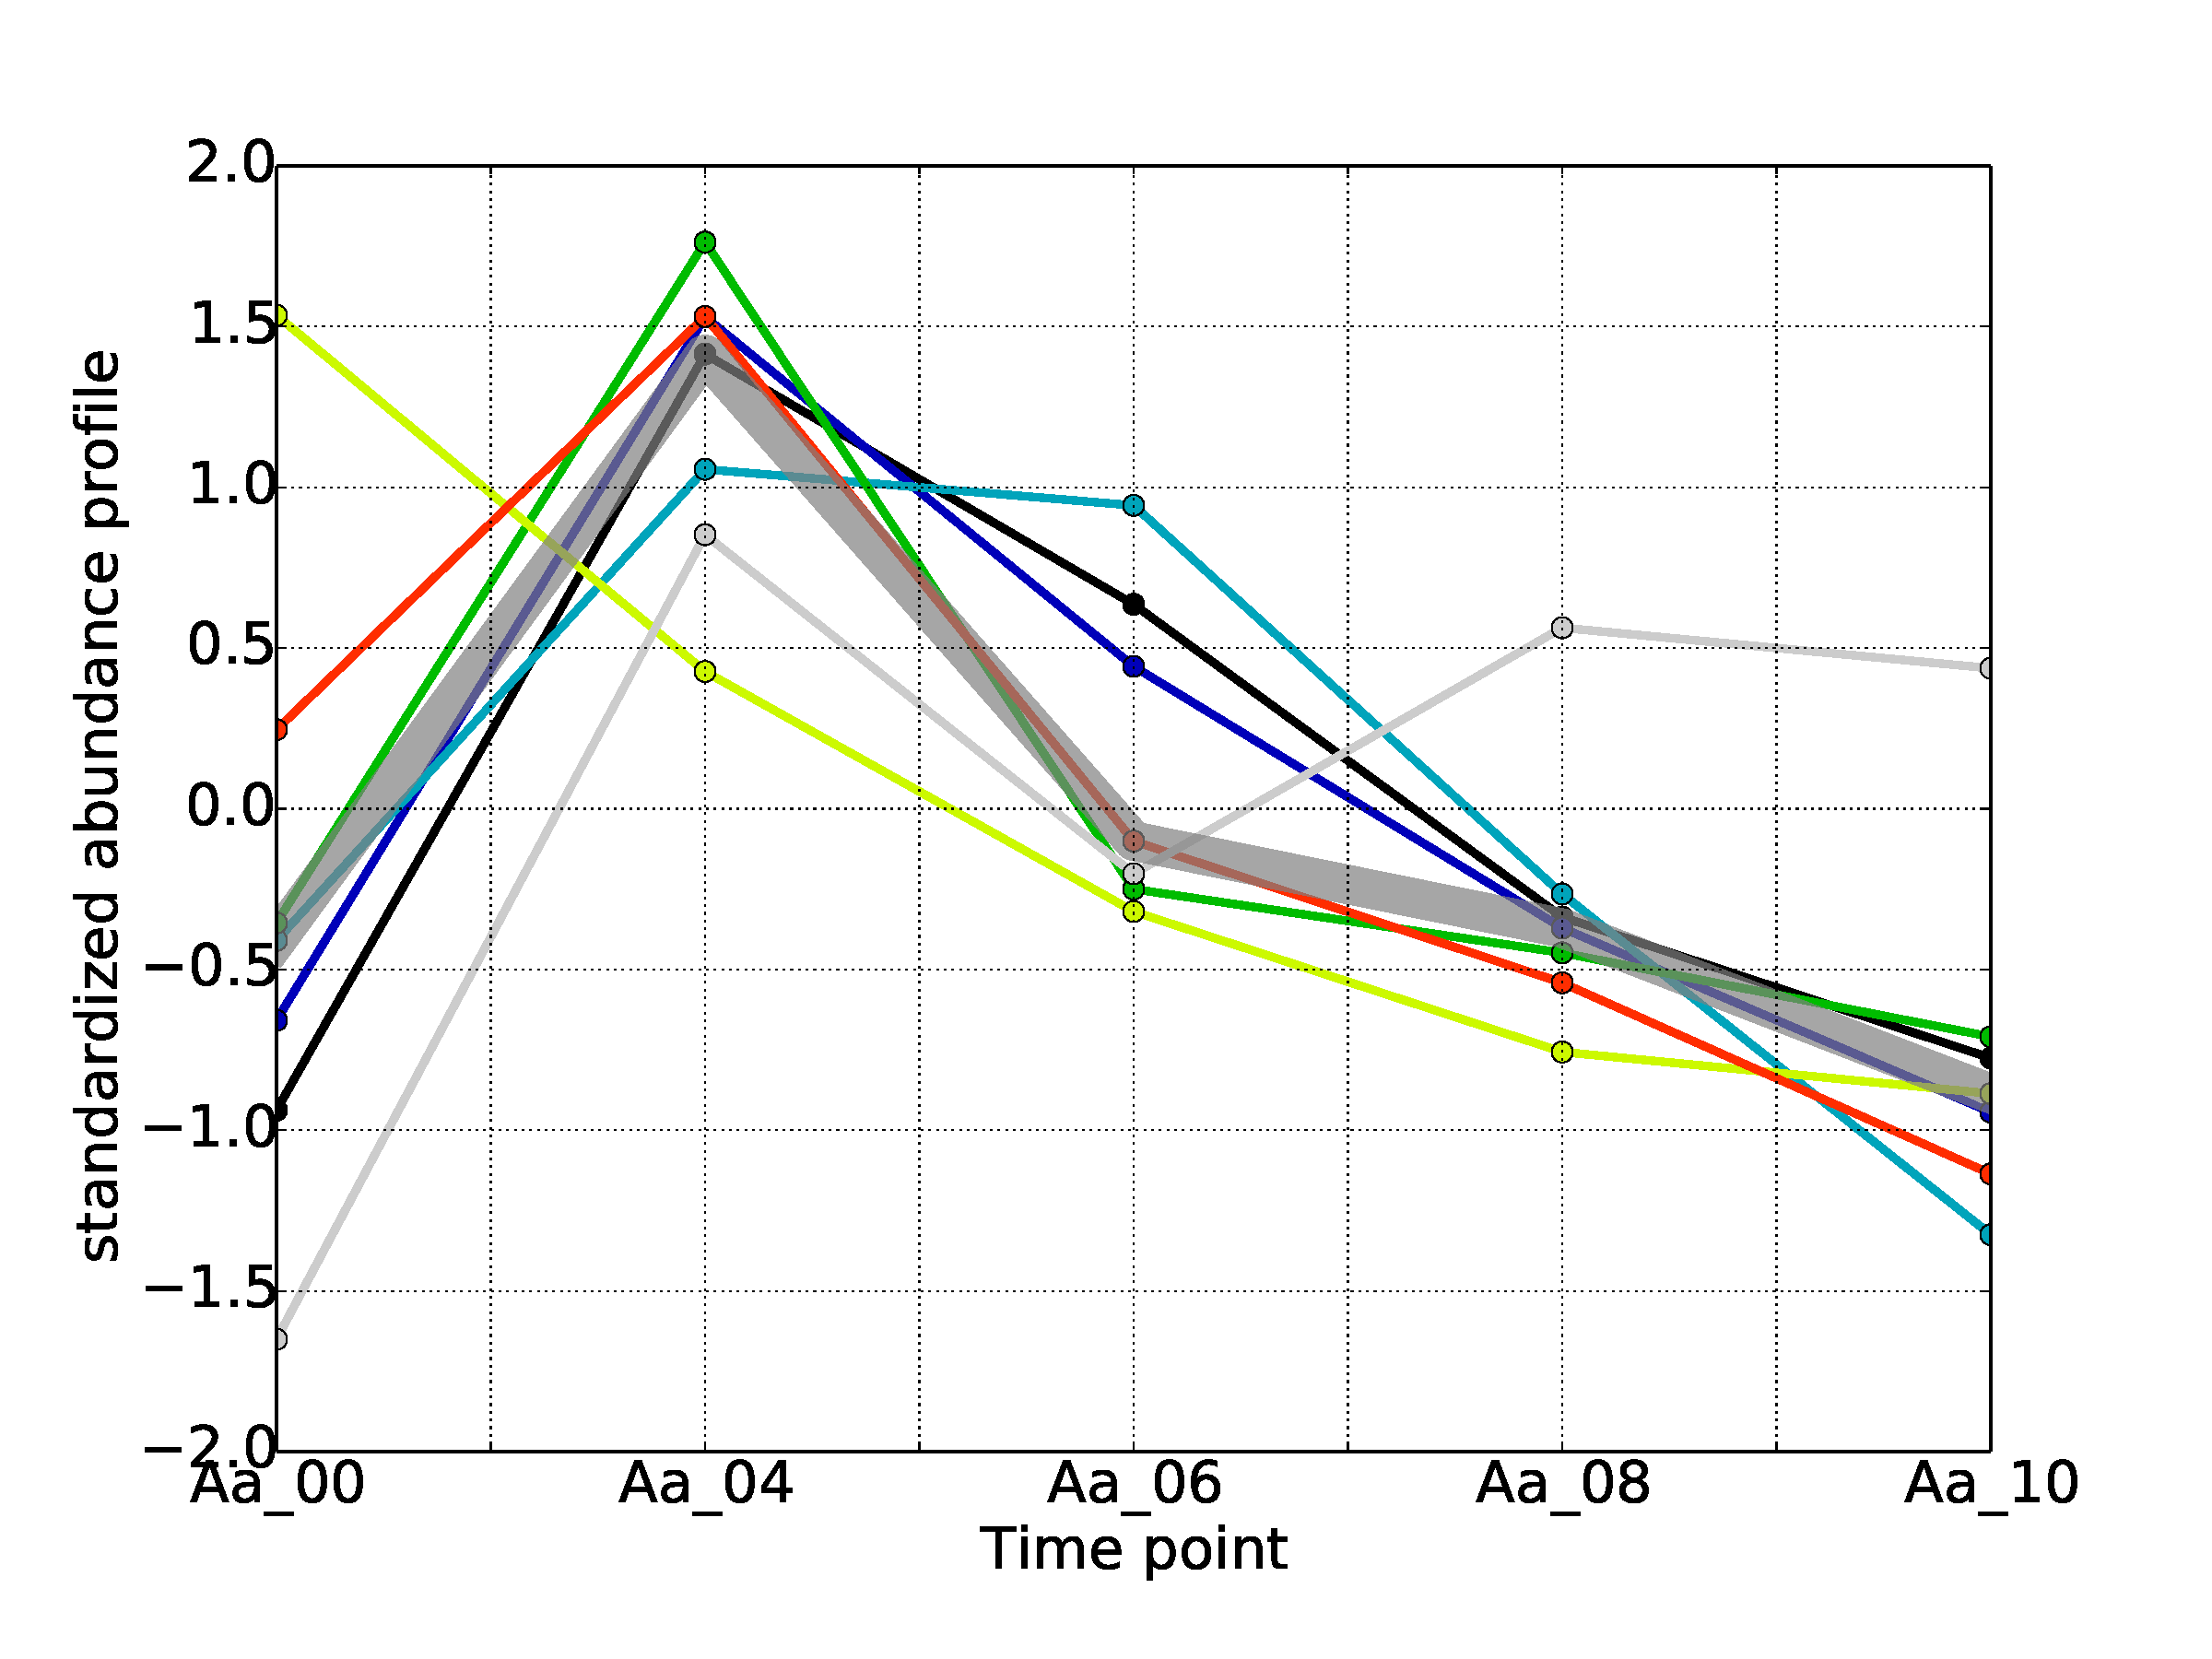
\includegraphics[width=.5\linewidth]{figures/figs/ecr_and_insects_ptci_20130918_orthodb7/upAt4_gene_profiles_from_cummerbund/Aa_upAt4_cls22_Ag_target_FPKMs_vb_orthos.pdf}}
%
\subcaptionbox{\label{fig:cluster22-Ag}}
{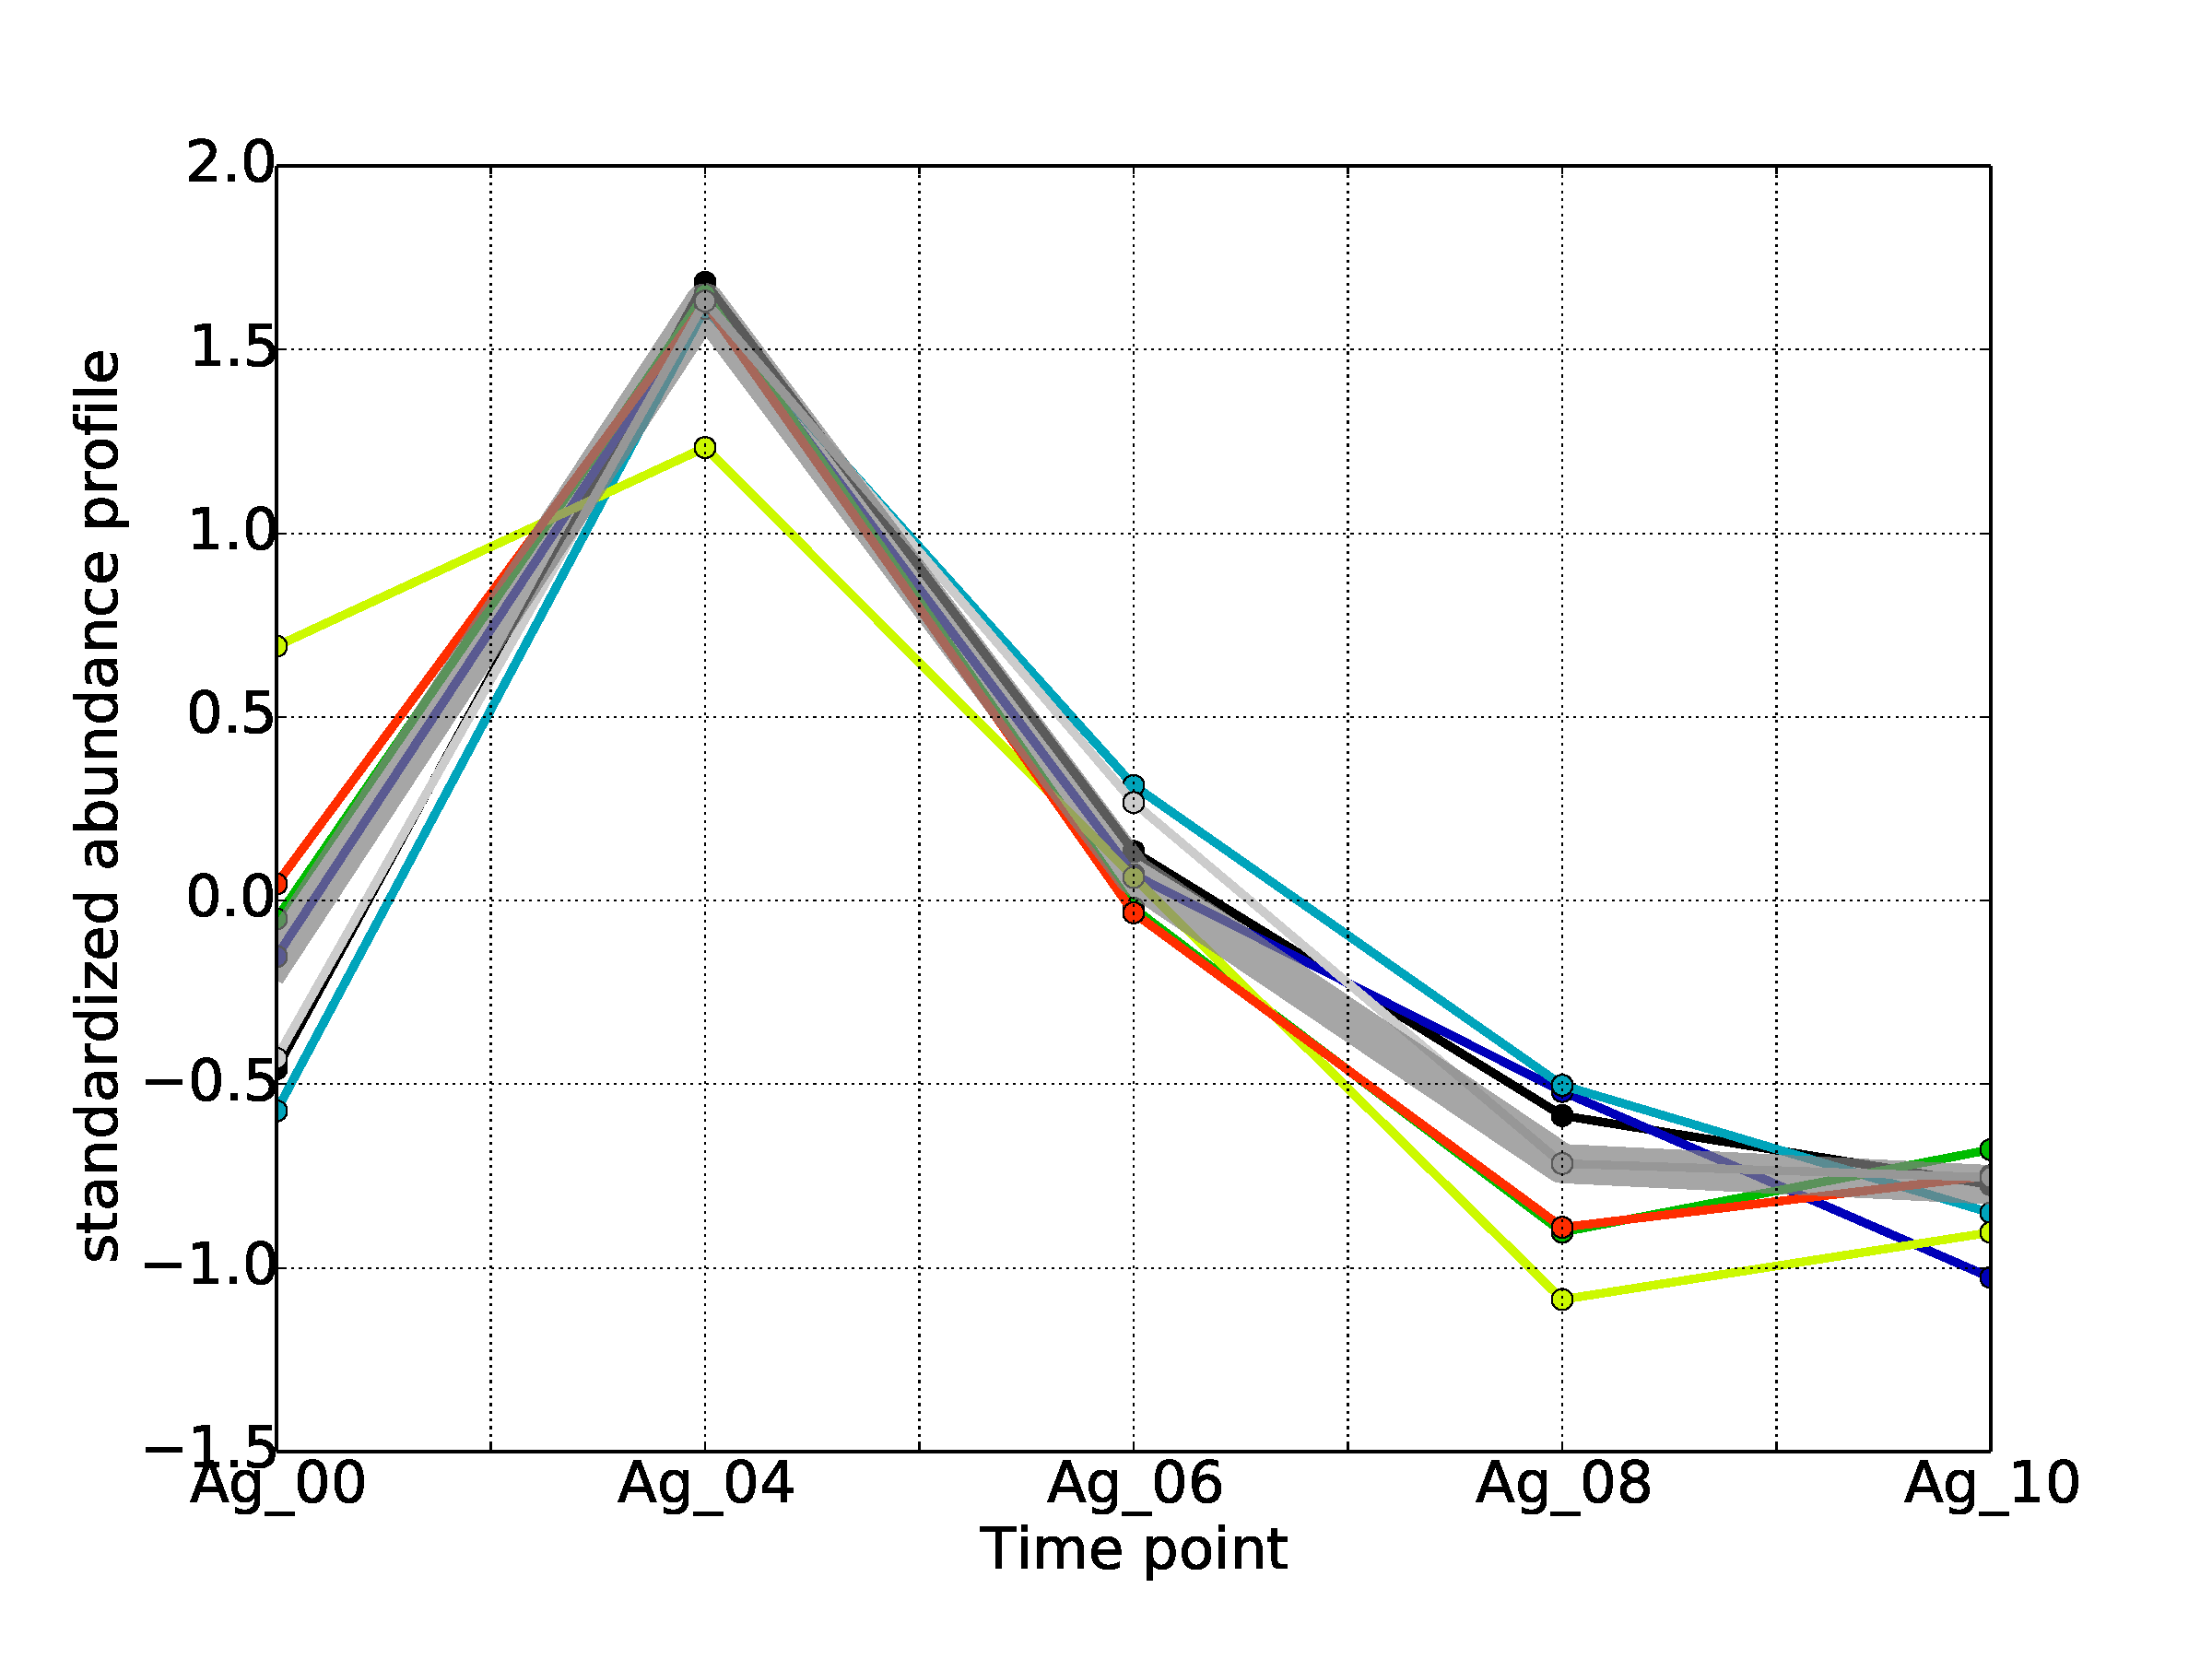
\includegraphics[width=.5\linewidth]{figures/figs/ecr_and_insects_ptci_20130918_orthodb7/upAt4_gene_profiles_from_cummerbund/Ag_upAt4_cls22_Ag_target_FPKMs_vb_orthos.pdf}}
%
\subcaptionbox{\label{fig:cluster22-Cq}}
{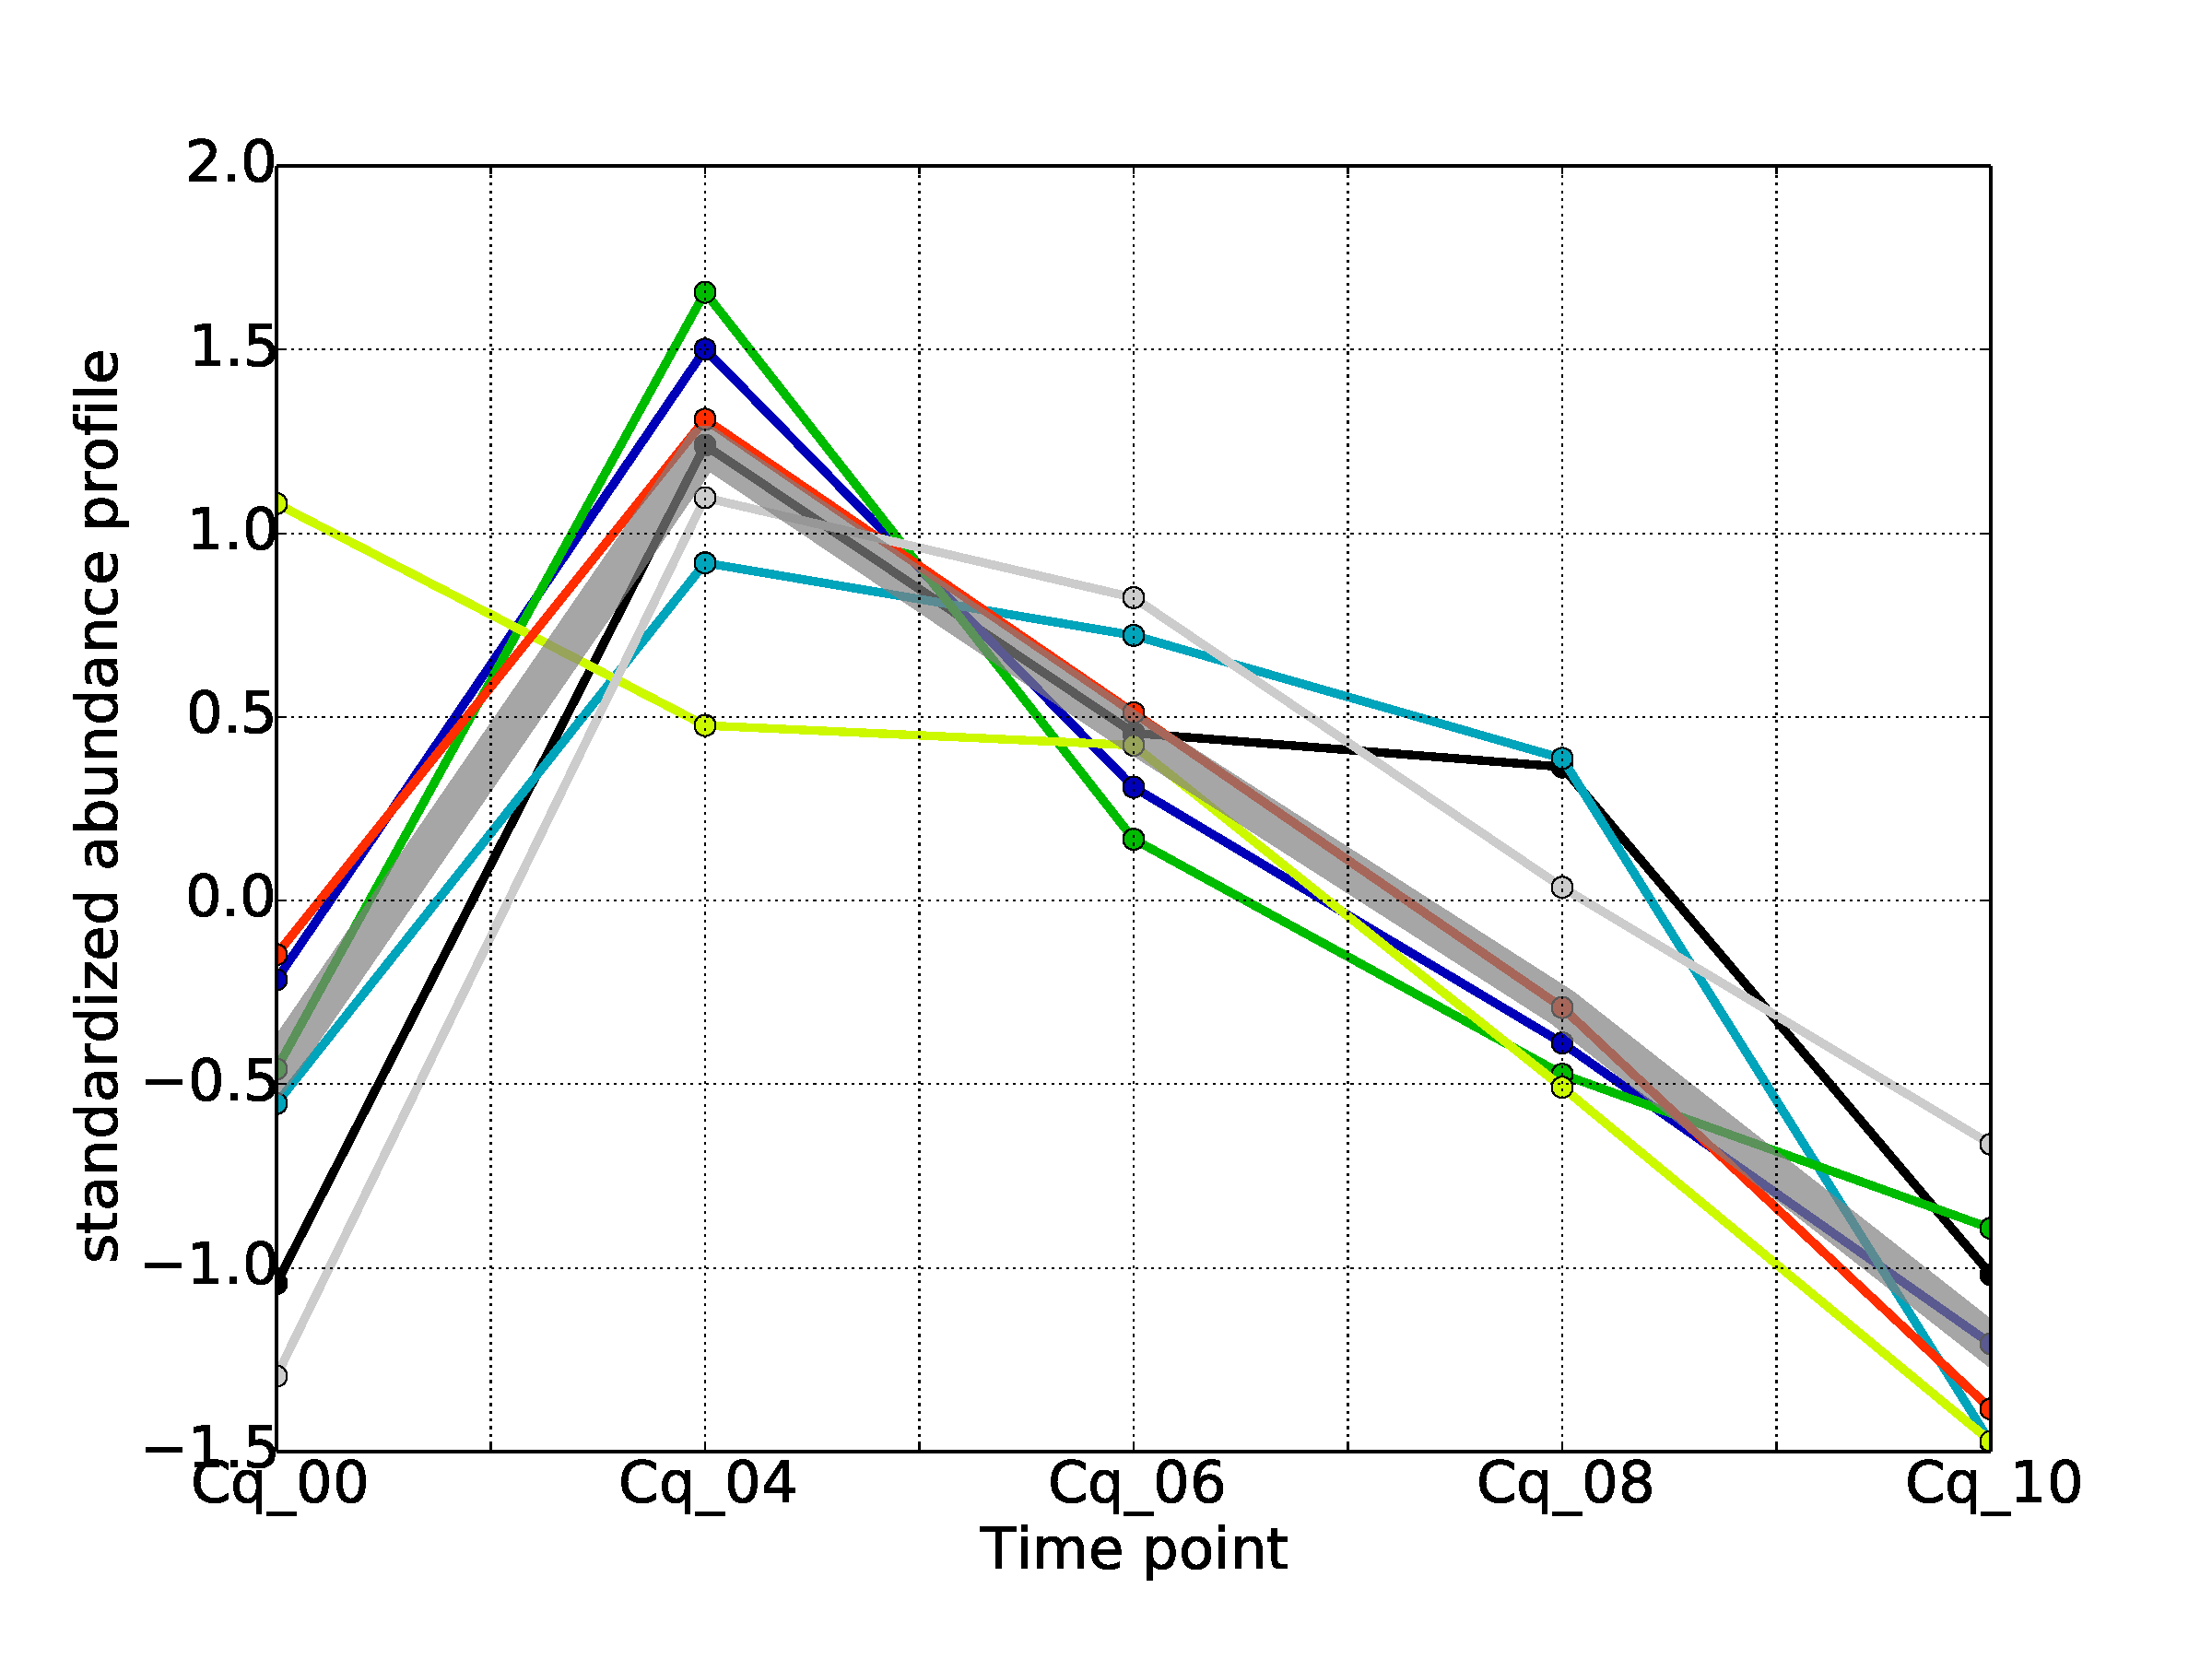
\includegraphics[width=.5\linewidth]{figures/figs/ecr_and_insects_ptci_20130918_orthodb7/upAt4_gene_profiles_from_cummerbund/Cq_upAt4_cls22_Ag_target_FPKMs_vb_orthos.pdf}}
% 
\caption[Orthologs of cluster 22]{\sf \textbf{Orthologs of cluster 22 (up at 4h):}\\
The same color scheme is used for each species which means that orthologs are given the same color in all three panels.
The thick, transparent gray line represents the median \gls{mAP} for the panel.
\textbf{(A)} \Aa.
\textbf{(B)} \Ag.
\textbf{(C)} \Cq.
}\label{fig:cluster22}
\end{figure}